
\clearpage

\section{Interacción radiación-materia}
\label{sec:INT}
En general este apartado se basa en dar una pequeña explicación de algunos fenómenos físicos relevantes en la interacción radiación materia, estos se basan en las diversas interacciones de partículas cargadas o fotones con átomos, existen otros procesos que son relevantes como la interacción de neutrones pero debido a que poco tienen que ver(por ahora) con el desarrollo de este trabajo no son incluidos.
\subsection{Interacciones de fotones en la materia}
 A menudo se asume que son solo cuatro los eventos relevantes para fotones al interactuar con átomos: dispersión de Compton, dispersión de Rayleigh, efecto fotoeléctrico, y producción de pares.
Pero en Realidad las interacciones más importantes de fotones con la materia son principalmente seis, las cuales son: dispersión de Compton, dispersión de Rayleigh, efecto fotoeléctrico, producción de nuclear de pares, producción electrónica de pares, y reacciones fotonucleares, esto es debido a que usualmente la producción de nuclear de pares junto a la producción electrónica de pares se manejan ambas bajo el nombre de producción de pares y los efectos de las reacciones fotonucleares son ignorados. A continuación se muestra una explicación sencilla de cada uno de ellos.

\subsubsection{Dispersión de Compton(Dispersión incoherente)}

El efecto Compton recibe su nombre en honor a Arthur Compton quien en 1922 fue la primer persona en realizar mediciones de una dispersión entre un fotón y un electrón libre, este fenómeno se basa en la interacción de un fotón con una energía $h\nu$ junto con un electrón débilmente ligado a un orbital de cierto átomo, cuando esto ocurre, se produce un fotón de energía menor $h\nu '$ y un electrón conocido como el electrón de Compton(dispersado) es expulsado del átomo con una energía cinética $E_k$, es pertinente mencionar que en estudios teóricos se asume que el electrón esta libre y estacionario\cite{Podgorsak}, generalmente es posible usar los cálculos de mecánica clásica con la conservación de energía y momento, sin embargo es importante entender la naturaleza cuántica del proceso, y en particular la transferencia de energía y la asignación de momento a un fotón implicada, los cálculos clásicos funcionan mientras, la velocidad no sea relativista, la energía de los fotones implicados no sea muy baja o el material tenga un numero atómico $Z$ muy alto, si alguna de estas situaciones se cumple es necesario realizar las correcciones apropiadas\cite{Edward}.\\
\begin{figure}[htbp]
    \centering
    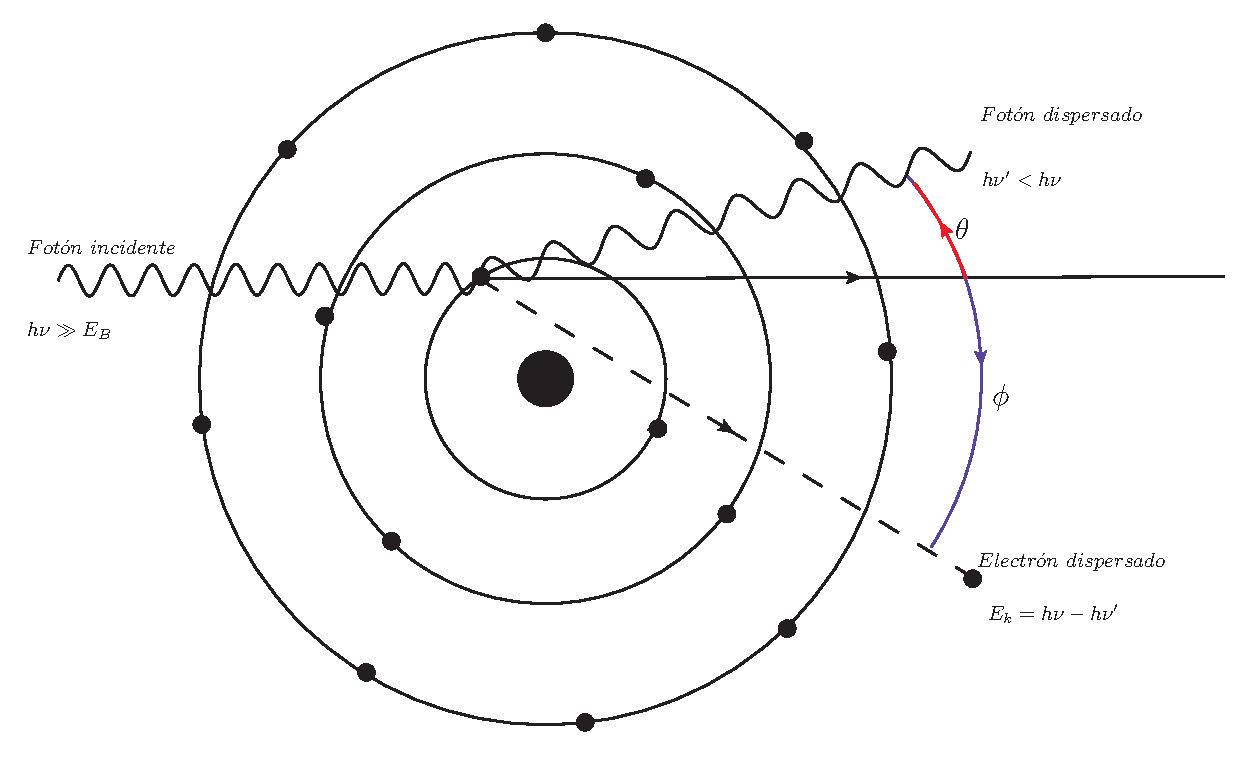
\includegraphics[width=.71\linewidth]{./Figures/compton1.eps}
    \caption[Efecto Compton]{Efecto Compton: un fotón incidente con energía $h\nu$ colisiona con un electrón débilmente ligado de un átomo produciendo un fotón con energía menor $h\nu '$ con angulo $\theta$ y a su vez es expulsando un electrón de Compton con energía cinética $E_k$ y angulo $\phi$}
    \label{fig:Compton}
\end{figure}

\subsubsection{Dispersión de Rayleigh(Dispersión coherente)}
Recibe el nombre de Rayleigh debido a el físico John W. Rayleigh quien en 1900 desarrollo una teoría para la dispersión de radiación electromagnética debido a átomos, este fenómeno ocurre principalmente con fotones a bajas energías $h\nu$ junto con un receptor que tenga numero atómico $Z$ alto, consiste en que un fotón incidente es dispersado cuando interactuá con alguno de los electrones ligados a un átomo, el átomo absorbe el momento transferido y el fotón es dispersado con un angulo $\phi$ y con una energía relativamente igual a la que tenía antes de la interacción, los ángulos de este fenómeno son relativamente pequeños dado que la energía impartida al átomo no produce ionización o excitación y este vuelve a su estado original después de la interacción\cite{Podgorsak}.
También se conoce como Dispersión coherente debido a que el fotón es dispersado por  la acción combinada de todo el átomo,debido a esto el evento es elástico en el sentido de que el fotón no pierde casi nada de su energía\cite{Frank}.

\begin{figure}[htbp]
    \centering
    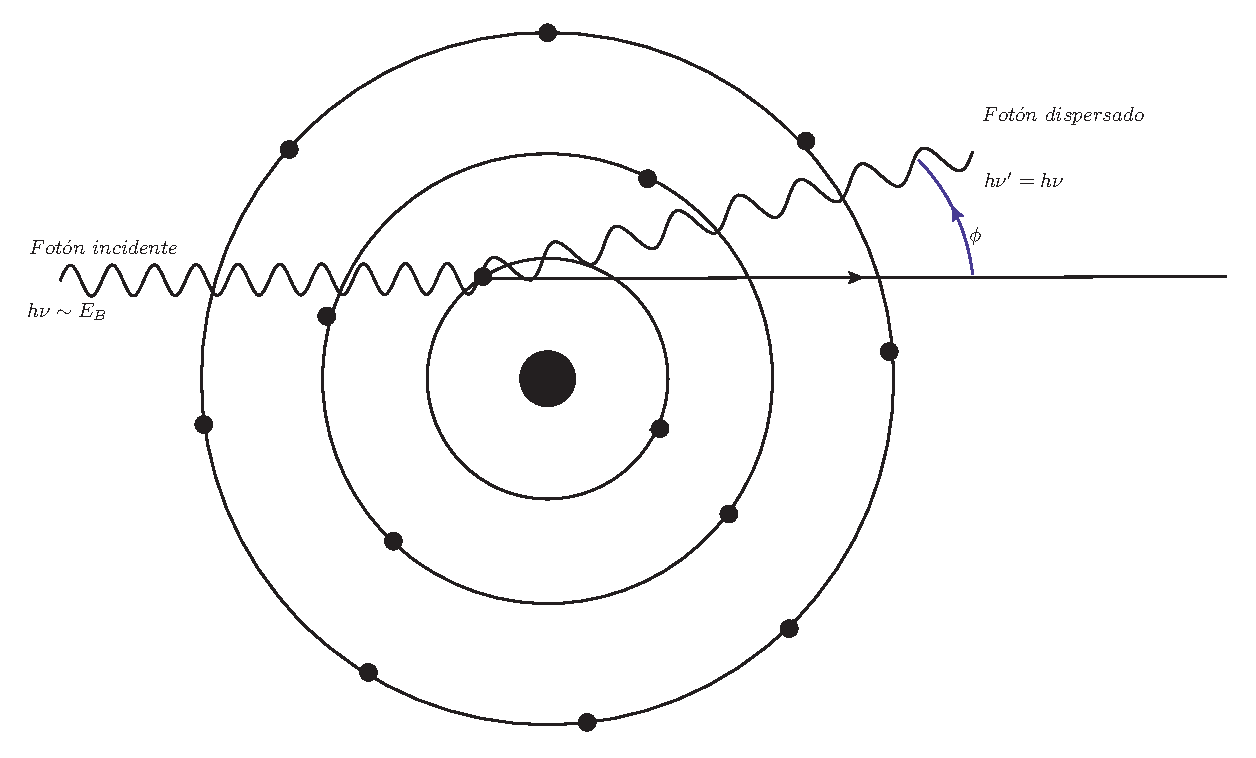
\includegraphics[width=.71\linewidth]{./Figures/Ray.eps}
    \caption[Dispersión de Rayleigh]{Dispersión de Rayleigh:un fotón incidente con energía $h\nu$ interactuá con un electrón ligado a un átomo, este fotón es dispersado con un angulo pequeño $\phi$ y una energía $h\nu '$ relativamente igual a $h\nu$ }
    \label{fig:DR}
\end{figure}


\subsubsection{Efecto fotoeléctrico}

Se conoce como efecto fotoeléctrico a la interacción entre un fotón y un electrón orbital fuertemente ligado a un átomo, el fotón incidente con energía $h\nu$ interactúa con el electrón del átomo, entonces es absorbido completamente y el electrón orbital conocido como fotoelectrón es expulsado con energía cinética $E_k=h\nu-E_B(K)$ Donde $E_B(K)$ es la energía de ionización del electrón, la vacante en el orbital es subsecuentemente tomada por con un electrón más alto y la energía de la transición del electrón sera emitida en la formá de un fotón característico(fluorescencia) o como un electrón de Auger.

A diferencia del efecto Compton el cual ocurre cuando un fotón interactuá con un electrón "libre"(débilmente ligado), el efecto fotoeléctrico sucede entre un fotón y un electrón "ligado fuertemente", la diferencia entre estos radica en la magnitud relativa de la energía del fotón $h\nu$ y la energía necesaria para remover un electrón de un átomo(energía de ionización) $E_B$ en vez de un valor absoluto de $h\nu$ o $E_B$, entonces cuando $E_B\ll h\nu$ se dice que el electrón esta débilmente ligado o libre y cuando  $E_B \lesssim h\nu$ se asume que el electrón esta fuertemente ligado\cite{Podgorsak}.


\begin{figure}[htbp]
    \centering
    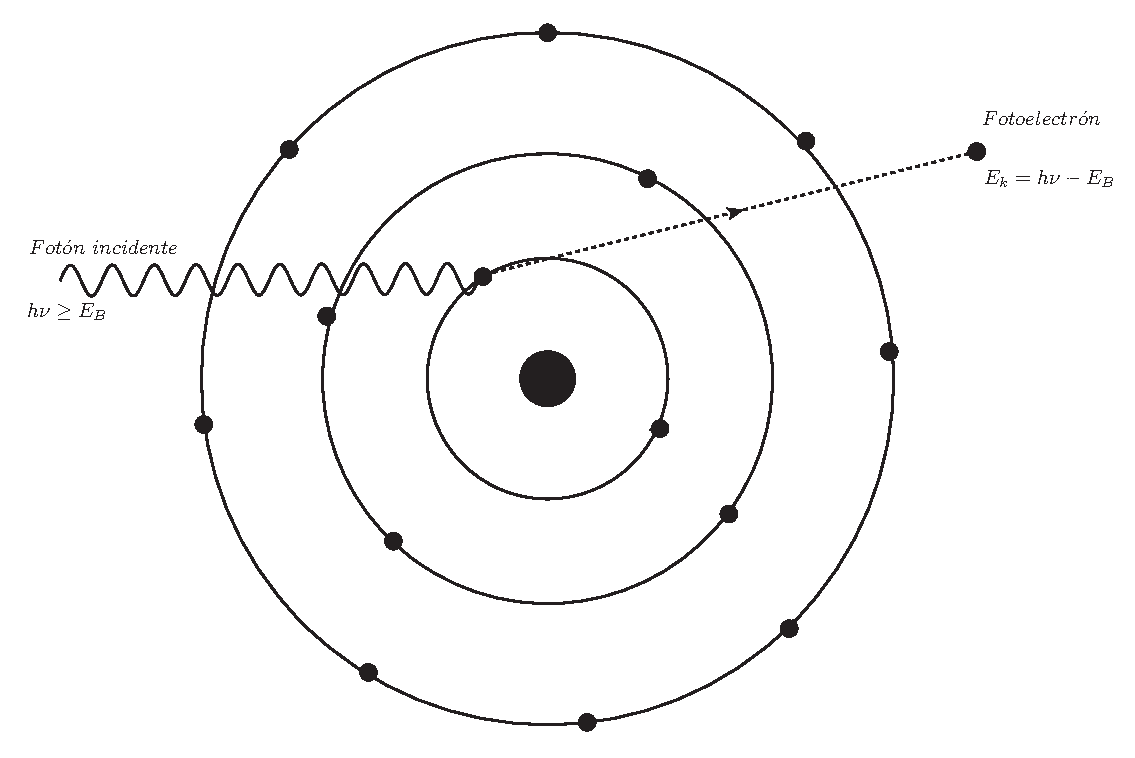
\includegraphics[width=.71\linewidth]{./Figures/fotoelec.eps}
    \caption[Efecto fotoeléctrico]{Efecto fotoeléctrico: un fotón incidente con energía $h\nu$ interactúa con el electrón del átomo, entonces es absorbido completamente y el electrón orbital conocido como fotoelectrón es expulsado con energía cinética $E_k$}
    \label{fig:FT}
\end{figure}

\subsubsection{Producción de pares}
Si un fotón con una energía mayor  1.02 MeV entra en un receptor, puede interactuar con los átomos de este por un proceso conocido como producción de pares, en este mecanismo de transferencia de energía el fotón al pasar cerca del átomo esta sujeto a efectos de campo fuerte debido al núcleo, y puede desaparecer y reaparecer como un par de electrones positivo y negativo.\cite{Edward}
Debido a que el momento $p_\nu$ antes de la interacción de producción de pares es mucho más grande que el momento total  $p_{pair}$ después de la interacción de producción de pares,  entonces el fotón debe poseer un exceso de momento que no puede ser absorbido por el par electrón-positrón, por tanto, debe ser absorbido por otro ente de colisión, sea el núcleo atómico, o un electrón orbital\cite{Podgorsak}, dada alguna de estas condiciones tenemos:
\paragraph{Producción nuclear de pares}
 Cuando el fotón interactuá con el núcleo atómico, este juega un rol más o menos pasivo, el estado del núcleo dispersado antes y después del evento es el mismo, excepto por un cambió en su energía cinética y momento. Simplemente un fotón se ha convertido en un electrón y un positrón\cite{Edward}.
\begin{figure}[htbp]
    \centering
    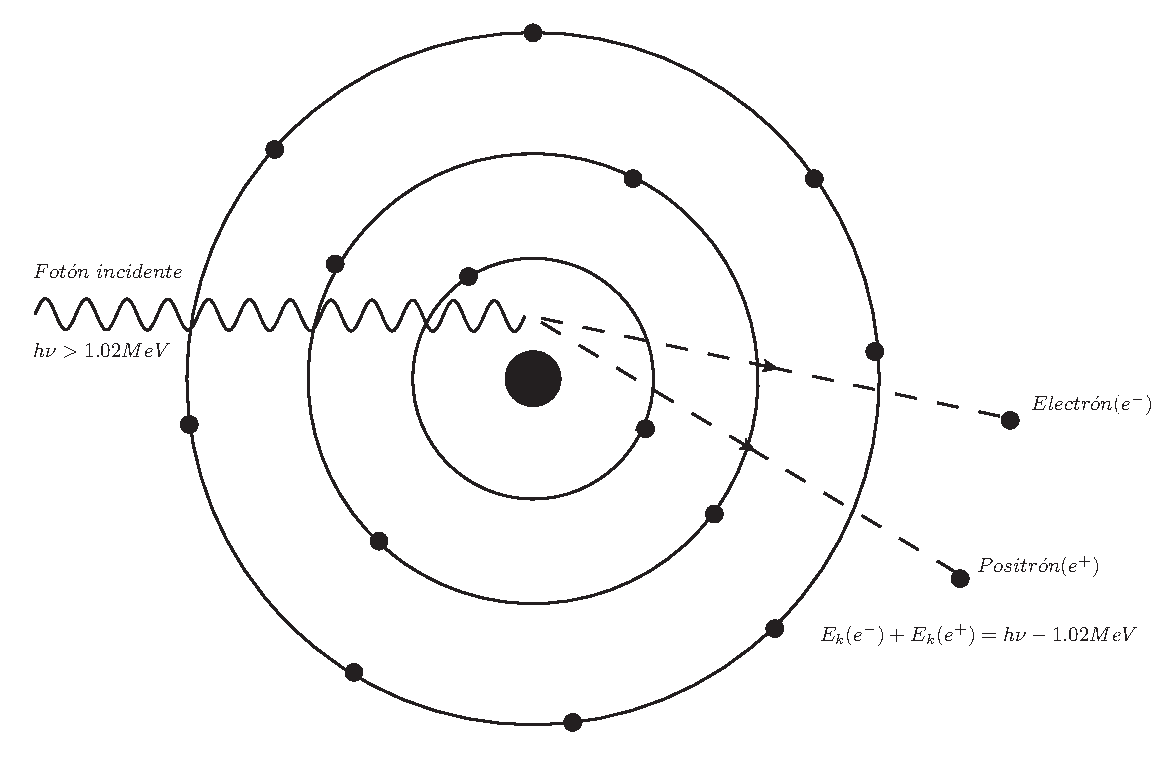
\includegraphics[width=.71\linewidth]{./Figures/nuclearpp.eps}
    \caption[Producción nuclear de pares]{Producción nuclear de pares: Un fotón experimenta una producción de pares estándar, electrón--Positrón}
    \label{fig:PN}
\end{figure}
\paragraph{Producción electrónica de pares}
 El fotón incidente interactúa con un electrón orbital, en lugar de con un núcleo atómico, debido a esto el electrón es dispersado, dado que tiene una masa pequeña, tomará una energía cinética significativa y aparecerá como un producto de la interacción. Además, un electrón y un positrón se generan como resultado de la desaparición del fotón incidente \cite{Edward}.
\begin{figure}[htbp]
    \centering
    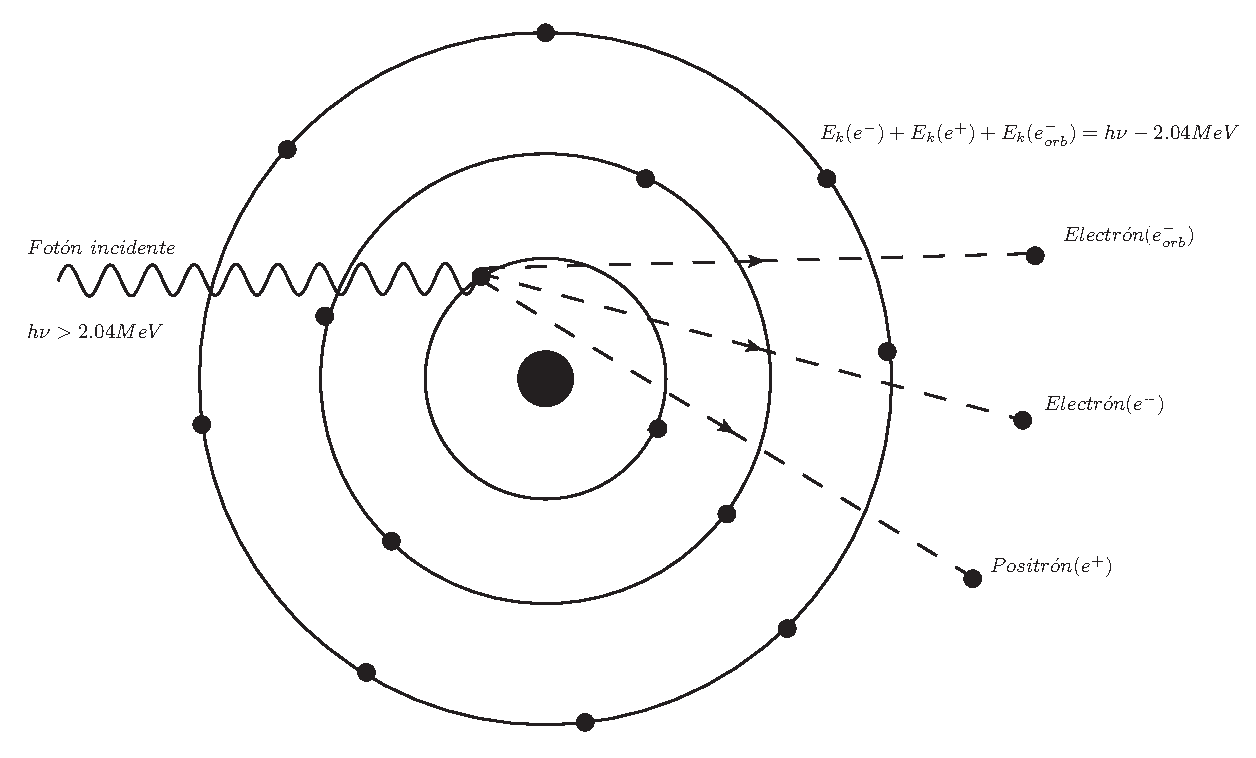
\includegraphics[width=.71\linewidth]{./Figures/electpp.eps}
    \caption[Producción electrónica de pares]{Producción electrónica de pares: Un fotón experimenta una producción de pares triple, un electrón dispersado--electrón--Positrón}
    \label{fig:PE}
\end{figure}

\paragraph{Reacciones fotonucleares}
 Usualmente este tipo de fenómeno también recibe el nombre de "fotodesintegración" ó "efecto nuclear fotoeléctrico", se basa en la interacción entre un fotón energético y un núcleo causando desintegración nuclear. En la reacción fotonuclear el núcleo absorbe el fotón y el resultado más probable es la emisión de un solo neutrón, aunque es posible que se emitan otras partículas como $\alpha$, rayos $\gamma$,más de un neutrón o fragmentos de fisión, aunque estos eventos son menos probables, un neutrón producido por este fenómeno se conoce como fotoneutrón\cite{Podgorsak}.

 \begin{figure}[htbp]
     \centering
     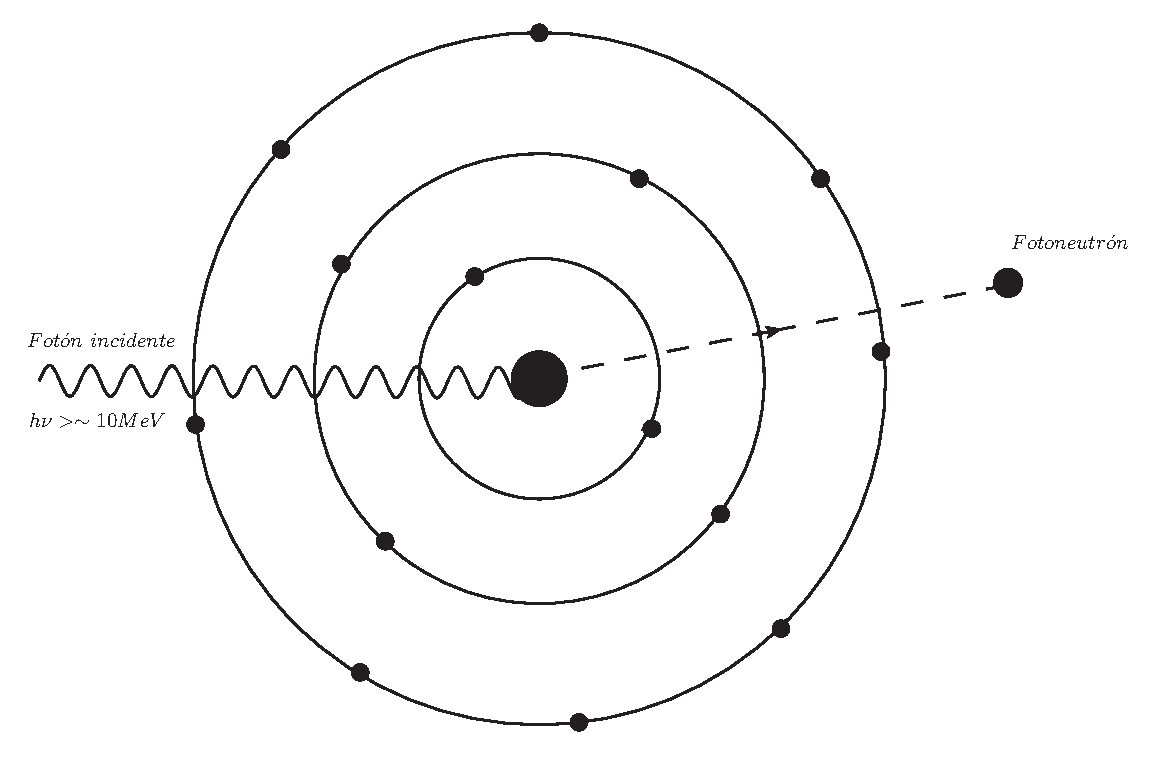
\includegraphics[width=.71\linewidth]{./Figures/fotoneu.eps}
     \caption[Reacción fotonuclear]{Reacción fotonuclear: Un fotón es absorbido por un núcleo atómico y este produce un fotoneutrón}
     \label{fig:RF}
 \end{figure}


\subsubsection{Interacciones de partículas cargadas en la materia}
A medida que una partícula viaja en un receptor experimenta interacciones de Coulomb con los núcleos y electrones de los átomos de este mismo, estas interacciones pueden ser divididas en tres categorías dependiendo del tamaño clásico del parámetro de impacto $b$ de la trayectoria de la partícula cargada comparado al radio clásico del átomo $a$ con el que la partícula interactuá.
\paragraph{Colisión de radiación($b\ll a$)}
Cuando el parámetro de impacto $b$ de una partícula cargada es mucho más pequeño que el radio $a$ del átomo, la partícula cargada interactuá más que todo con el núcleo y experimenta dispersión elástica o inelástica junto con un posible cambio en la dirección del movimiento. En la mayoría de los casos se presenta dispersión elástica en cuyo caso la partícula es dispersada por el núcleo pero solo sufre una pequeña perdida de su energía cinética, sin embargo un pequeño porcentaje de estas interacciones son inelasticas y pueden resultar en perdida significante de energía para la partícula cargada acompañada por la emisión de fotones de rayos-x, este tipo de interacción se conoce como colisión de bremsstrahlung\cite{Podgorsak}.


\paragraph{Bremsstrahlung}
Bremsstrahlung es un tipo de fotón de rayos-x producido cuando partículas ligeras experimentan interacción radioactiva inelástica con núcleos de átomos de dado receptor, en esta interacción la partícula presenta ralentización
 dando una fracción significante de energía cinética al fotón\cite{Frank}. Las partículas cargadas de interés para la física medica y dosimetría se pueden clasificar en dos categorías:
\begin{enumerate}
  \item Partículas ligeras cargadas: electrones $e-$ y positrones $e+$, ambos pueden producir fotones bremsstrahlung debido a su masa relativamente pequeña\cite{Podgorsak}.
  \item  Partículas pesadas cargadas: protones $p$, deuterones $d$, partículas alfa $\alpha$, iones pesados tales como $Li^+$,$Be^+$,$C+$,$Ne+$, etc. producen una cantidad insignificante de fotones bremsstrahlung\cite{Podgorsak}.
\end{enumerate}


Bremsstrahlung es la palabra en alemán para designar radiación de frenado.

\begin{figure}[htbp]
   \centering
   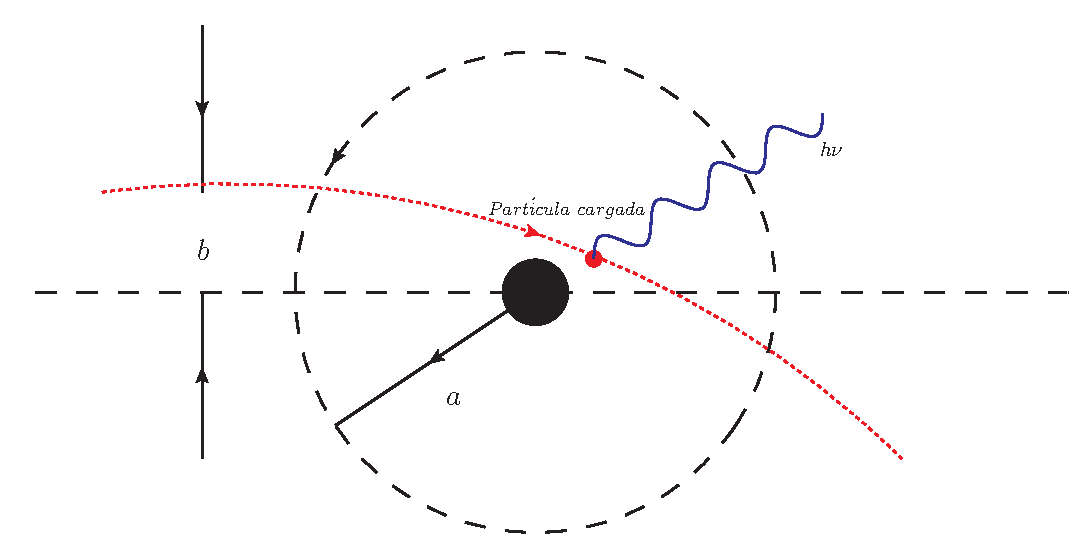
\includegraphics[width=.65\linewidth]{./Figures/radiacol.eps}
   \caption[Colisión de radiación]{Colisión de radiación(producción de bremsstrahlung)}
   \label{fig:B}
\end{figure}


\paragraph{Colisión fuerte($b\approx a$)}
Cuando el parámetro $b$ de la trayectoria de una partícula cargada sea aproximadamente del orden del radio $a$ del átomo,la partícula cargada puede tener un impacto directo de Coulomb con un electrón de un orbital, a este fenómeno se le conoce como Colisión fuerte en el cual se transfiere una cantidad significante de energía de la partícula al electrón, luego de la interacción el electrón deja el átomo como un rayo $\gamma$, el numero de colisiones fuertes que  experimenta  una partícula cargada moviéndose en un receptor es generalmente pequeño, sin embargo la transferencia de energía asociada es relativamente grande\cite{Podgorsak}.


\begin{figure}[htbp]
   \centering
   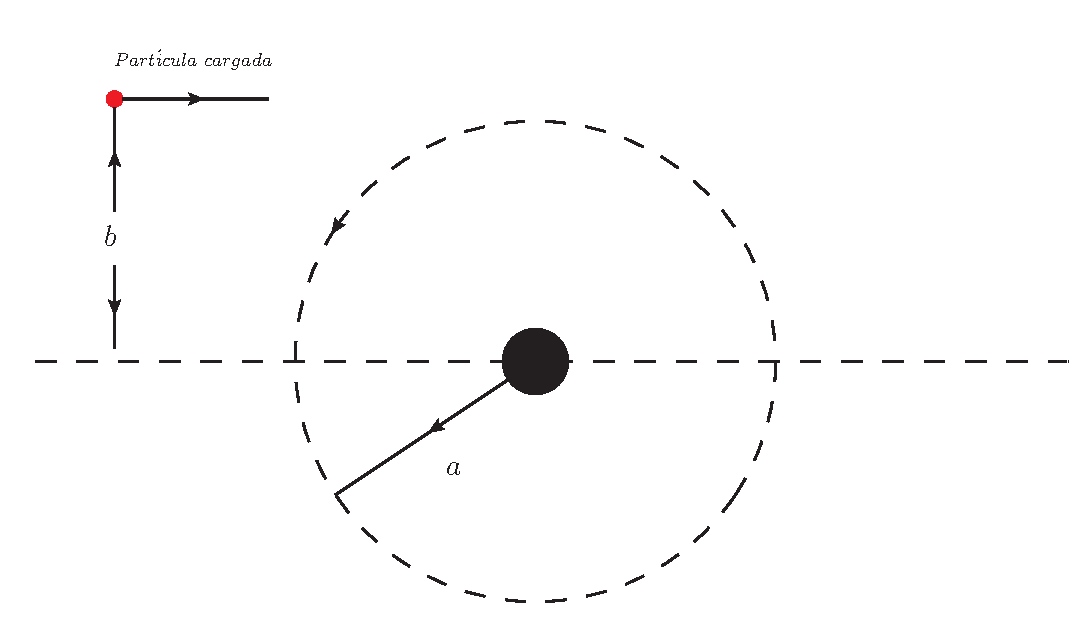
\includegraphics[width=.65\linewidth]{./Figures/hardcoli.eps}
   \caption{Colisión fuerte}
   \label{fig:cf}
\end{figure}

\paragraph{Colisión debil($b\gg a$)}
Cando el parámetro $b$ de la partícula cargada es mucho más grande que el radio $a$ del átomo, la partícula cargada interactuá con todo el átomo el cual se compone de electrones ligados, la energía transferida por la partícula cargada en este evento a los electrones ligados es muy pequeña, sin embargo el numero de estas interacciones es bastante grande, y debido a esto la partícula pierde mucha energía, estas mini-interacciones pueden causar polarización atómica, excitación o ionización mediante la remoción de un electrón de valencia, este fenómeno recibe el nombre de colisión débil o colisión suave\cite{Podgorsak}.

\begin{figure}[htbp]
   \centering
   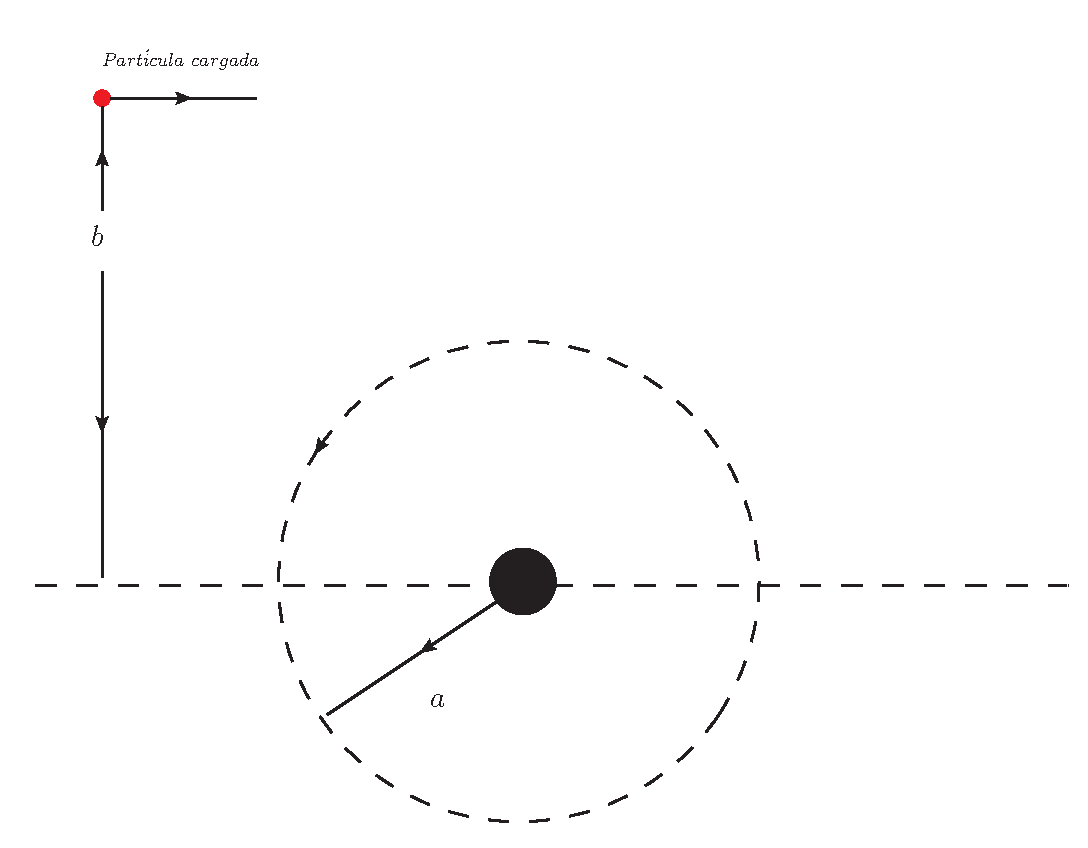
\includegraphics[width=.65\linewidth]{./Figures/softcoli.eps}
   \caption{Colisión débil o suave}
   \label{fig:cd}
\end{figure}
